\section{Softwarekonzept} \label{sec:softwarekonzept}

\subsection{Anforderung Software} \label{subsec:anforderungSoftware}

Die Software soll das Frequenzverhalten und die Einfügungsverluste von CM und DM des EMI-Filters simulieren können. Das Werkzeug soll insbesondere mit einer Empfindlichkeitsanalyse die Auswirkungen der parasitäreren Parameter auf die Einfügungsverluste des Filters darstellen. Die parasitären Filterparameter können in einem Bereich von ± 30\% variiert werden. Der Filter wird mit Hilfe von CM- und DM äquivalenten Schaltungsmodellen berechnet. Um die Auswirkungen der Parametervariation besser sichtbar zu machen, wird der Frequenzbereich des Filters in 3 Sektoren aufgeteilt: 0 kHz bis 500 kHz, 500 kHz bis 5 MHz und 5 MHz bis 30 MHz. Das Klassendiagramm ist in der Abbildung \ref{fig:Klassendiagramm} ersichtlich.

\subsection{Softwarestruktur} \label{subsec:softwarestruktur}

Die Software wird mit dem Model-View-Controller Entwurfsmuster (MVC Design Pattern) \cite{MVCDesignPattern} strukturiert. Durch diese Strukturierung ist es weitgehende möglich die Daten und dessen graphischer Repräsentation zu trennen. Dies vereinfacht Wartungsarbeiten und die Wiederverwendbarkeit von Programmteile. Die Struktur ist in die drei Teilen Modell(engl. model), Präsentation(engl. view) und Steuerung(engl. controller) unterteilt

\subsection{Softwareelemente} \label{subsec:softwareelemente}

\subsubsection{Eingabefenster} \label{subsubsec:eingabefenster}

Das Eingabefenster ist dazu da, die einzelnen parasitären Filterparameter einzustellen und die Toleranz von ± 30\% mit einem Schieberegler zu variieren (F6, Tabelle:\ref{tab:ziele}) . Die  Textfelder werden vor Fehleingaben geschützt (B1, Tabelle:\ref{tab:ziele}) und unterstützt spezielle Eingabeformen (z.B 10 milli=10m) (G2, Tabelle:\ref{tab:ziele})

\subsubsection{CM/DM Plot} \label{subsubsec:CM_DMplot}

Um die Berechnungen zu visualisieren werden 2 Plots für CM und DM verwendet(G4, Tabelle:\ref{tab:ziele}) Die Plots sind für die bessere Darstellung in 3 Frequenzbereiche aufgeteilt:0 kHz bis 500 kHz, 500 kHz bis 5 MHz und 5 MHz bis 30 MHz(G3, Tabelle:\ref{tab:ziele}). Mit einem Rechtsklick auf den Plot können verschiedene Optionen ausgewählt werden. So können die Eigenschaften (Farbe, Darstellung, Schrift usw.) und der Zoom individuell eingestellt werden(Fehlt bei Zielen). Der Plot kann auch direkt in eine .png Datei abgespeichert oder gedruckt werden(B2, Tabelle:\ref{tab:ziele}). Diese Optionen sind in der Abbildung \ref{fig:PlotSettings} ersichtlich.

\begin{figure}[H]
	\centering
	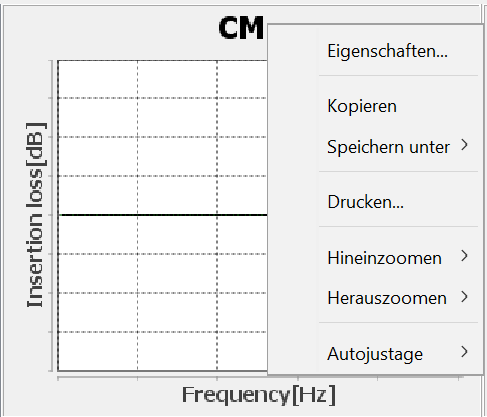
\includegraphics[width=4cm]{PlotSettings.png}
	\caption{Ploteinstellungen}
	\label{fig:PlotSettings}
\end{figure} 


\subsubsection{Filtertabelle} \label{subsubsec:filtertabelle}

Für das Wunschziel (B3, Tabelle:\ref{tab:ziele}) kann in einer Filtertabelle alle erstellte Filterprofile dargestellt und verwaltet werden.  Mit einer Checkbox können einzelne Profile im Plot aus- bzw. eingeblendet werden. Zudem kann bei jedem Filterprofil einen Namen hinzugefügt werden. Die Werte der parasitären Filterparameter des ausgewählten Filterprofils werden in das Eingabefenster geladen und können dort verändert werden. Mit den Shortcuts Backspace and Delete können ausgewählte Profile gelöscht werden.

\subsubsection{Buttonfenster} \label{subsubsec:buttonfenster}

Im Buttonfenster können Filterprofile in die Filtertabelle geladen oder entfernt werden. (TODO:Zielverweis) Mit dem Button Add werden die eingegebene parasitären Filterparameter in einem neuen Filterprofil gespeichert. Mit dem Button Remove wird das ausgewählte Filterprofil gelöscht. Der Button dient als alternative zu den Shortcuts.


\subsubsection{Menu} \label{subsubsec:menu}

Im Menu können verschiedene Optionen ausgewählt werden. Diese sind ebenfalls alle mit einem Shortcut aufrufbar. (TODO:Zielverweis Ziel Menu)

\bigskip
\shorthandoff{"}
\paragraph{File} \label{para:file}
Im Menupunkt "File" können Filterprofile gespeichert und geladen werden. (B4, Tabelle:\ref{tab:ziele}) Bei beiden Optionen wird der Explorer geöffnet um die .txt Datei im gewählten Verzeichnis abzulegen oder zu holen. In der Option Exit kann das Programm geschlossen werden. Dieser Menupunkt ist in der Abbildung \ref{fig:GUIFile} \nameref{fig:GUIFile} dargestellt.

\begin{figure}[H]
	\centering
	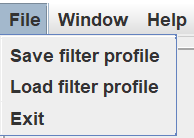
\includegraphics[width=4cm]{GUIFile.png}
	\caption{Menuoption File}
	\label{fig:GUIFile}
\end{figure}

\bigskip

\paragraph{Simulation} \label{para:simulation}
Im Menupunkt "Simulation" kann die Simulationsart Monte Carlo ausgewählt werden(F8, Tabelle:\ref{tab:ziele}). Es öffnet sich ein neues Fenster in dem der Parameter, die Toleranz und die Anzahl Messungen eingestellt werden kann. Dieser Menupunkt ist in der Abbildung \ref{fig:GUISimulation} dargestellt.

\begin{figure}[H]
	\centering
	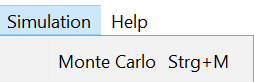
\includegraphics[width=4cm]{GUISimulation.png}
	\caption{Menuoption Simulation}
	\label{fig:GUISimulation}
\end{figure}

\newpage

\paragraph{Help} \label{para:Help}
Im Menupunkt "Help" können die beiden CM- und DM äquivalenten Schaltungsmodelle, die zur Berechnung verwendet werden, in einem seperaten Fenster dargestellt werden(G5, Tabelle:\ref{tab:ziele}). Dieser Menupunkt ist in der Abbildung \ref{fig:GUIHelp} \nameref{fig:GUIHelp} dargestellt.

\begin{figure}[H]
	\centering
	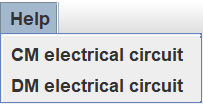
\includegraphics[width=4cm]{GUIHelp.png}
	\caption{Menuoption Help}
	\label{fig:GUIHelp}
\end{figure}
\shorthandon{"}

\subsection{Programmablauf} \label{subsec:programmablauf}

Der folgende Programmablauf ist auf die Maximallösung bezogen. In dieser Lösung sind alle Wunschziele(Tabelle:\ref{tab:ziele}) vorhanden.

Nach dem Aufstarten des Programmes kann der Benutzer über die Programmoberfläche (\ref{fig:GUI} \nameref{fig:GUI}) seine Simulationen starten.
Am Anfang ist ein default Filter initialisiert. Dieser ist in der Filtertabelle eingetragen, jedoch sind die parasitären Filterparameter im Eingabefenster noch undefiniert. Der Benutzer kann diese nun definieren und die berechneten Einfügungsverluste von CM und DM des EMI-Filters werden im Plot dargestellt. Mit dem Button Add wird der Filter abgespeichert und ein neuer Filter kann definiert werden. Es können somit mehrere Filter gleichzeitig dargestellt werden. 

Um die Filter richtig zu verwalten ist es möglich in der Filtertabelle über die Checkbox einzelne Filter im Plot ein und auszublenden. Ebenfalls können sie spezifisch benannt werden. Der Plot und die einzelnen Kurven können mit einem Rechtsklick auf den CM/DM Plot individuell angepasst und auch exportiert werde. Wird ein Filter nicht mehr benötigt kann er in der Filtertabelle angewählt und mit dem Button Remove entfernt werden. Damit der Benutzer nicht jedesmal die Filterprofile einstellen muss, können diese über File/Save filterprofil in einer .txt Datei abgespeichert werden. Bei einem Neustart des Programmes kann über File/Load filterprofile die Filterprofile wieder geladen werden. 

Um die Auswirkungen einzelner parasitären Filterparameter besser zu analysieren, kann unter Simulation/Monte Carlo eine Monte Carlo Simulation gestartet werden. Es wird ein neues Fenster geöffnet in dem der Filterparameter, die Toleranz und die Anzahl Berechnungen eingestellt werden können. Jede Berechnung wird als einzelner Filter in die Filtertabelle geladen. Um nachzuschauen wo welche Filterparameter sich in der Schaltung befindet, können unter Help/CM electrical circuit und CM electrical circuit die Ersatzschaltungen, von der die Berechnungen ausgehen, angeschaut werden. Das Programm wird über File/Exit oder beim Schliessen des Fensters beendet.

\newpage

\subsubsection{Klassendiagramm} \label{subsubsec:Klassendiagramm}

\begin{figure}[H]
	\centering
	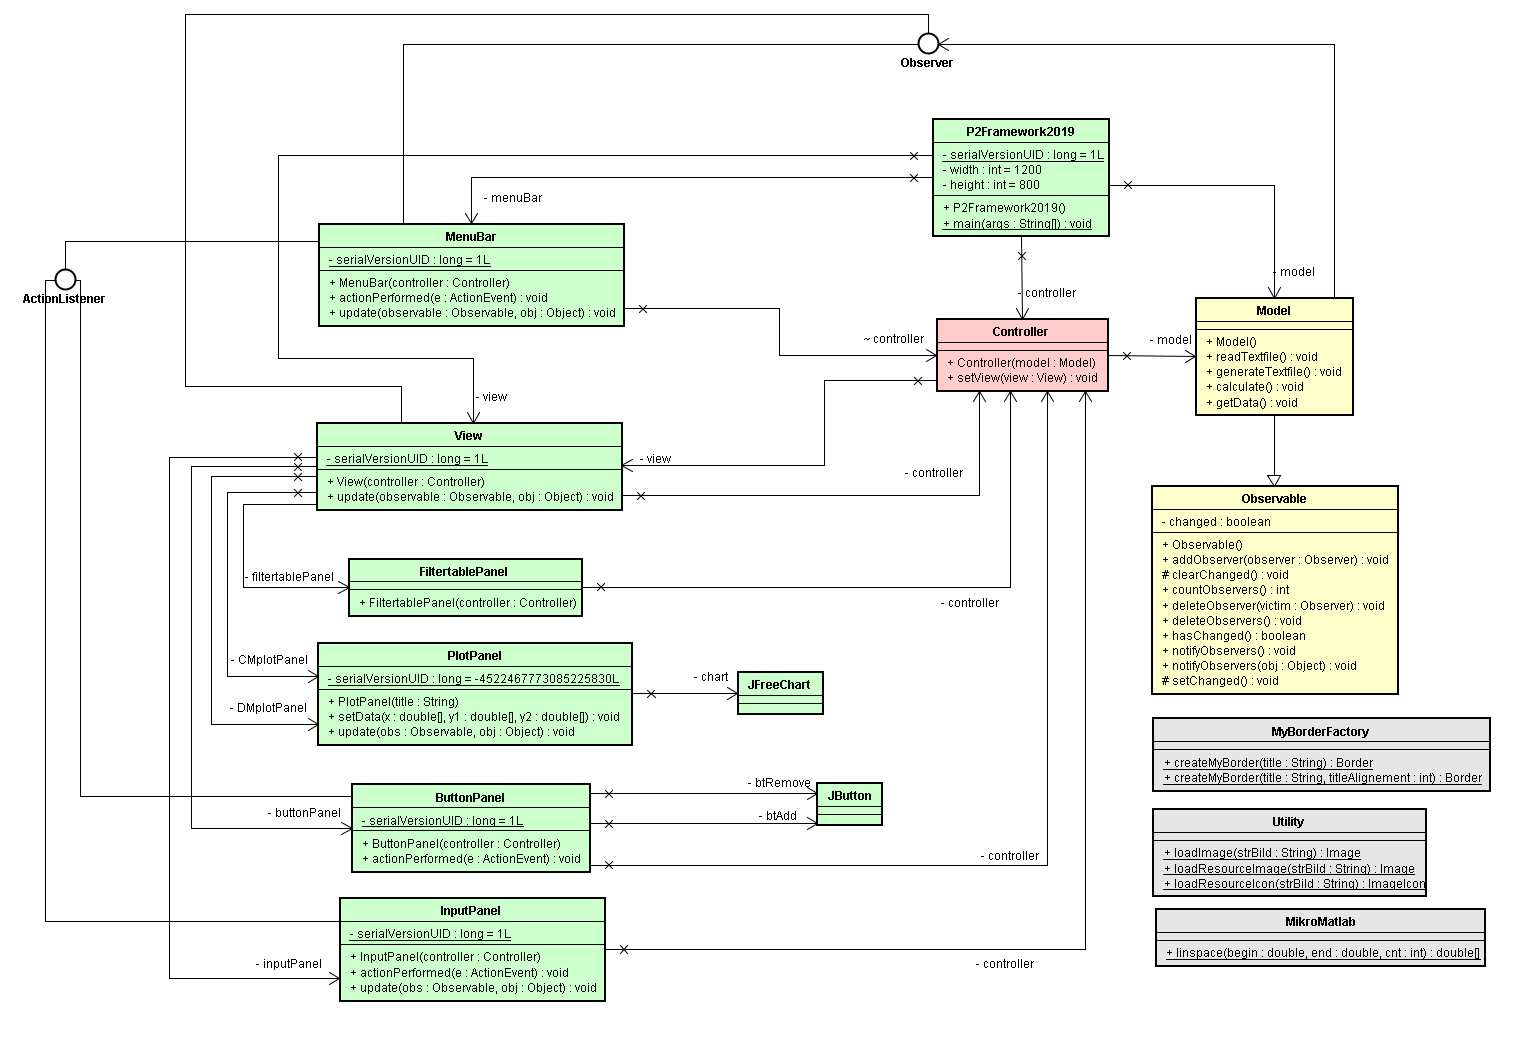
\includegraphics[width=16cm]{Klassendiagramm.png}
	\caption{Klassendiagramm}
	\label{fig:Klassendiagramm}
\end{figure} 

\newpage

\subsection{GUI} \label{subsec:GUI}

Die GUI wird in 5 Teilbereiche aufgeteilt: Menu, Filtertabelle, CM/DM Plot, Buttonfenster und Eingabefenster. In der Abbildung \ref{fig:GUI} \nameref{fig:GUI} ist die Benutzerfläche des Programms dargestellt.

\begin{figure}[H]
	\centering
	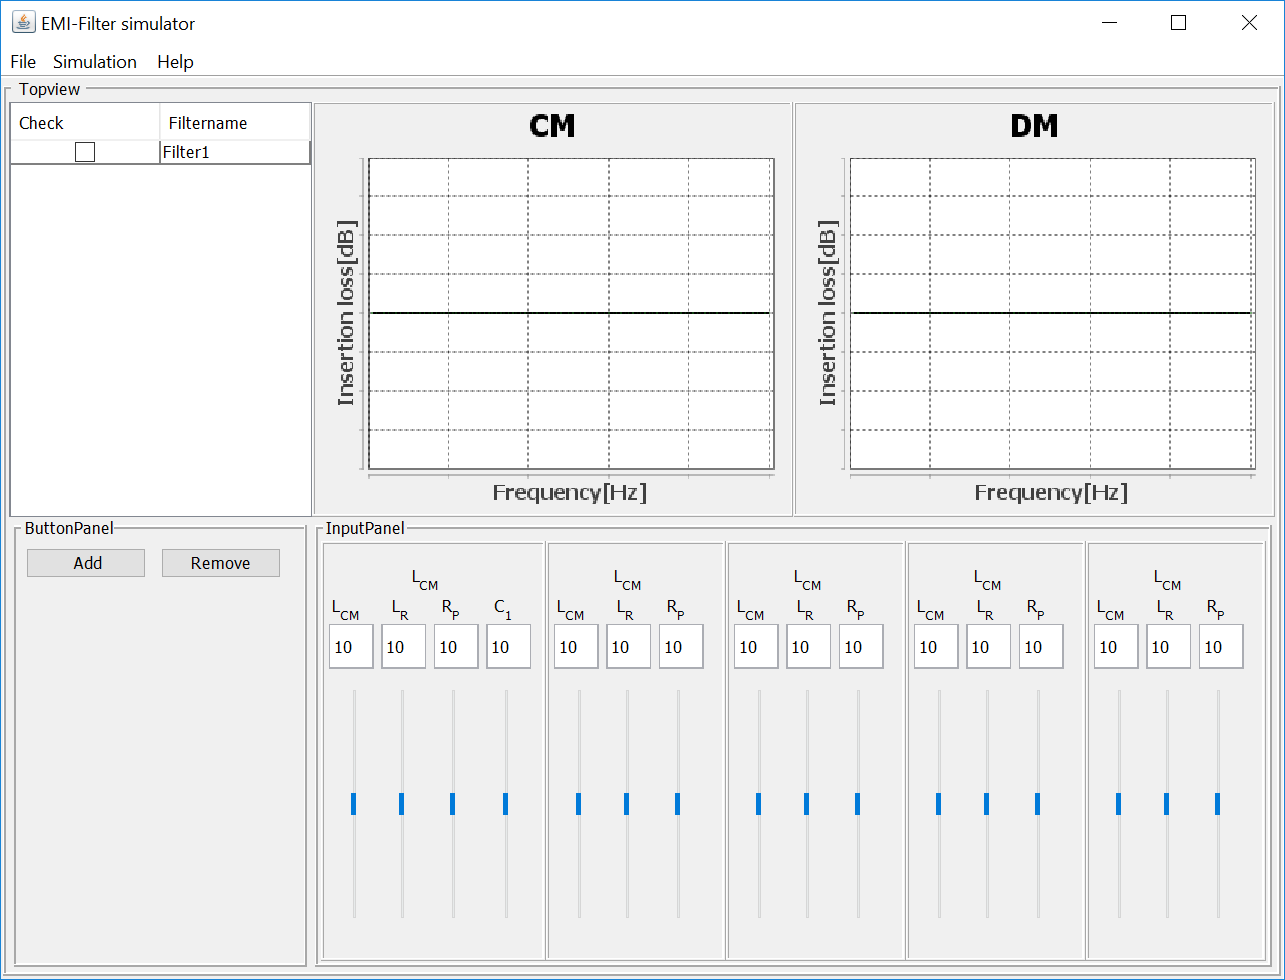
\includegraphics[width=10cm]{GUI.png}
	\caption{GUI}
	\label{fig:GUI}
\end{figure}



\subsection{Libraries} \label{subsec:Libraries}

In der Software werden folgende Libraries verwendet:

\textbf{Swing}: Mit dem vorinstallierten Swing Framework von Java wird die GUI aufgebaut.
\textbf{JFreeChart}: Die Berechnungen werden mit JFreeChart grafisch also Plot dargestellt. \cite{jfreechart}
\textbf{Apache Math Commons} Die Apache Math Commons Library beinhaltet wichtige Mathematikfunktionen, wie rechnen mit Komplexen Zahlen usw. \cite{apache}
\textbf{Engineering Text Fields} Die von Prof. Dr. Richard Gut zur Verfügung gestellte Klasse verhindert Fehleingaben und vereinfacht die Eingabe von Zahlen (nano,piko...)

\newpage
